\section*{Exercise 4A}

\begin{table}[h]
\begin{tabular}{cc}
\hline
\multicolumn{1}{|l|}{\textbf{Event A}} & \multicolumn{1}{l|}{\textbf{Event B}} \\ \hline
\multicolumn{1}{|c|}{$\varphi{16}$}                 & \multicolumn{1}{c|}{$\varphi{3}$}                 \\ \hline
\multicolumn{1}{|c|}{$\varphi{5}$}                  & \multicolumn{1}{c|}{$\varphi{18}$}                 \\ \hline
\multicolumn{1}{|c|}{$\varphi{17}$}                 & \multicolumn{1}{c|}{$\varphi{6}$}                 \\ \hline
\multicolumn{1}{|c|}{$\varphi{15}$}                 & \multicolumn{1}{c|}{$\varphi{6}$}                 \\ \hline
                                       &                                       \\
                                       &                                      
\end{tabular}
\end{table}

\begin{figure}[h]
    \centering
    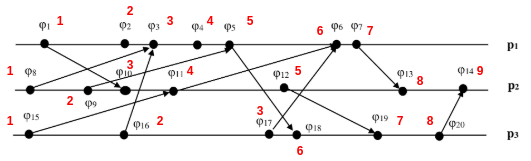
\includegraphics[width=\textwidth]{fig/4b.png}
\end{figure}


\begin{figure}[h]
    \centering
    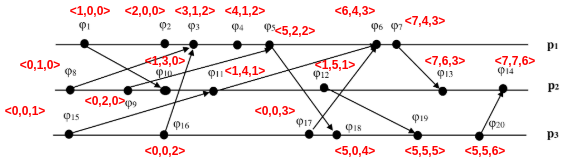
\includegraphics[width=\textwidth]{fig/4c.png}
\end{figure}

\section*{Exercise 4B(i)}
Let's have an example with two processes P1 and P2. P1 send a message
M1 to P2. The message M1 was delivered after a later-sent application
message. Because of this reordering, the recorded global state is
inconsistent

\section*{Exercise 4B(ii)}
By recording the messages in the process states, we can ignore
flushing channels. In this model, the original Chandy-Lamport
algorithm that assumes FIFO channels is:

\begin{lstlisting}[style=mycode]
Process 0: 
	Send "SS" to self

Process i: 
	when receive "SS" for first time (from pj):
		  record state
		  send "SS" to all neighbors
		  for each neighbor except pj wait for "SS"
\end{lstlisting}

To accommodate non-FIFO channels, we just have to ensure that the
delivery of the snapshot message does not get moved after the delivery
of subsequent messages. For this reason, we block sending application
messages until the snapshot is complete. We define a set BLOCK for
each process p. For each process q in BLOCK, p will block all sends to
q until q is no longer in BLOCK.

\begin{lstlisting}[style=mycode]
Process0: 
	send "SS" to self
Process i: 
	when receive "SS" for first time (from pj):
		  record state
		  BLOCK = all neighbors - { pj }
		  send "SS" to all neighbors
		  while (BLOCK != 0):
			  when receive "SS" (from pk)
			  BLOCK = BLOCK - { pk }
\end{lstlisting}
